\subsection{Méthode de Jacobi par blocs}
Afin d'obtenir une évaluation de la borne maximale de l'accélération qu'il est possible d'obtenir sur une machine donnée, nous proposons de connaître l'accélération obtenue par une méthode de Jacobi par blocs et de la comparer à notre solution.
%
Dans cette méthode, nous considérons le cas où chaque coeur effectue la factorisation ILU(0) d'un sous bloc diagonal de la matrice.
%
Cette méthode de préconditionnement induit une factorisation et une résolution triangulaire totalement indépendante sur chaque coeur.
%
Elle n'est évidemment pas équivalente numériquement à effectuer une factorisation ILU de toute la matrice.
%
Plus on utilise de coeurs, plus ce préconditionneur est inefficace numériquement\cite{domain_decomp}.
%
Mais l'intérêt cette évaluation est que l'accélération obtenue donne une borne supérieure de l'accélération de la factorisation ILU sur la matrice complète.
%
Cette borne existe puisqu’individuellement chaque coeur utilise une factorisation dont la bande passante mémoire est approximativement égale à celle de l'algorithme ILU globale.


Malgré un parallélisme idéal, nous n'obtenons pas une accélération parfaite pour la factorisation ILU(0) (Fig.~\ref{fig:res_facto_mpi}).
%0
De plus, les performances de la résolution triangulaire sont basses malgré un parallélisme total (Fig.~\ref{fig:res_trsv_mpi}).
%
C'est un problème que l'on rencontre souvent dans les codes d'algèbre linéaire creuse.
%
Si l'on compare les accélérations obtenues avec celles obtenues avec l'agrégation de tâches, on peut voir des résultats légèrement meilleurs pour la méthode Jacobi par blocs.
%
Notre solution d'agrégation n'est pas optimale, mais cette différence d'accélération n'est pas seulement due à la granularité du calcul.

%   (-_-)   %
\begin{figure}
  \centering
  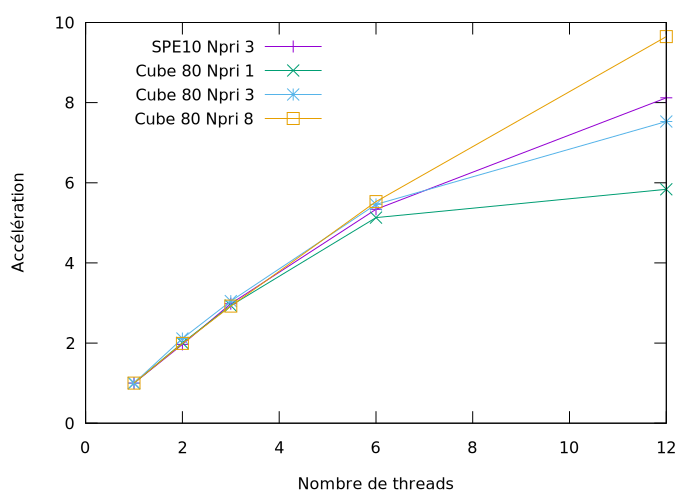
\includegraphics[width=0.7\textwidth]{res_facto_mpi}
  \caption{Performance de la factorisation ILU(0) sur 12 coeurs en utilisant une méthode de Jacobi par blocs.}
  \label{fig:res_facto_mpi}
\end{figure}
%   (-_-)   %
\begin{figure}
  \centering
  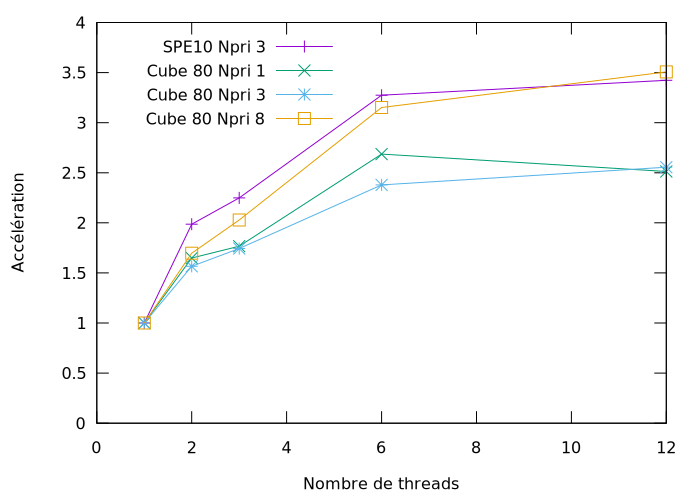
\includegraphics[width=0.7\textwidth]{res_trsv_mpi}
  \caption{Performance de la résolution triangulaire sur 12 coeurs en utilisant une méthode de Jacobi par blocs.}
  \label{fig:res_trsv_mpi}
\end{figure}

Il est nécessaire de regarder du côté de la bande passante mémoire pour trouver des explications.
%
Nous allons maintenant mesurer cette bande passante à l'aide des compteurs matériels.
%
La bande passante utilisée lors de la factorisation parallélisée par une méthode de Jacobi par blocs est au mieux de 16~Go/s, avec les threads nous utilisons 12~Go/s de bande passante locale dont 5~Go/s de bande passante distante.
%
Cette bande passante distante est le résultat des effets NUMA.
%
Dans le cas des processus MPI utilisée par la méthode Jacobi par blocs, chaque processus a son propre espace mémoire et la localité des données est assurée sous réserve d'un placement statique et optimal des processus.
%
Mais dans le cas des threads, l'espace mémoire est partagé entre deux bancs mémoires et si les accès mémoire ne sont pas optimisés, il y aura des transferts entre les bancs NUMA.
%
Ces transferts auront pour effet d'augmenter la latence des accès mémoire et de réduire le nombre de cycles d'horloge par instruction (CPI\footnote{Clock Per Instruction}), ici on a un CPI de 0,75 pour la version MPI contre 1,08 pour la version threadée (résultats obtenus avec les compteurs matériels).
%
L'explication de la différence de performance entre ces deux versions se situe au niveau de la mémoire, on est limité par la bande passante.
%% +-----------------------------+----------+----------+MPI12
%% |           Metric            |  core 0  |  core 6  |
%% +-----------------------------+----------+----------+
%% |     Runtime (RDTSC) [s]     | 115.248  | 115.248  |
%% |    Runtime unhalted [s]     | 124.295  | 124.907  |
%% |         Clock [MHz]         | 3050.46  | 3053.54  |
%% |             CPI             | 0.751758 | 0.753133 |
%% | Memory bandwidth [MBytes/s] | 15905.1  | 15835.6  |
%% | Memory data volume [GBytes] | 1833.04  | 1825.02  |
%% |  Remote Read BW [MBytes/s]  | 10.3343  | 23.2978  |
%% | Remote Write BW [MBytes/s]  | 0.913861 | 1.61113  |
%% |    Remote BW [MBytes/s]     | 11.2482  | 24.9089  |
%% +-----------------------------+----------+----------+

%% +-----------------------------+----------+----------+MPI6(2*3)
%% |           Metric            |  core 0  |  core 6  |
%% +-----------------------------+----------+----------+
%% |     Runtime (RDTSC) [s]     | 155.807  | 155.807  |
%% |    Runtime unhalted [s]     | 168.391  | 168.976  |
%% |         Clock [MHz]         | 3055.54  | 3055.33  |
%% |             CPI             | 0.544832 | 0.510243 |
%% | Memory bandwidth [MBytes/s] |  11664   | 11561.2  |
%% | Memory data volume [GBytes] | 1817.34  | 1801.31  |
%% |  Remote Read BW [MBytes/s]  | 6.52392  | 31.9625  |
%% | Remote Write BW [MBytes/s]  | 0.532458 | 1.44266  |
%% |    Remote BW [MBytes/s]     | 7.05638  | 33.4051  |
%% +-----------------------------+----------+----------+
%% +-----------------------------+----------+----------+MPI6(1*6)
%% |           Metric            |  core 0  |  core 6  |
%% +-----------------------------+----------+----------+
%% |     Runtime (RDTSC) [s]     | 226.632  | 226.632  |
%% |    Runtime unhalted [s]     | 0.422044 | 245.002  |
%% |         Clock [MHz]         | 2518.14  | 3046.49  |
%% |             CPI             | 1.14334  | 0.728566 |
%% | Memory bandwidth [MBytes/s] | 13.2691  | 16633.6  |
%% | Memory data volume [GBytes] |  3.0072  | 3769.69  |
%% |  Remote Read BW [MBytes/s]  |  5.9309  | 1.91099  |
%% | Remote Write BW [MBytes/s]  | 0.362203 | 0.167456 |
%% |    Remote BW [MBytes/s]     |  6.2931  | 2.07845  |
%% +-----------------------------+----------+----------+

%% +-----------------------------+---------+---------+THREAD_NO_AGG
%% |           Metric            | core 0  | core 6  |
%% +-----------------------------+---------+---------+
%% |     Runtime (RDTSC) [s]     | 1761.37 | 1761.37 |
%% |    Runtime unhalted [s]     | 1679.57 | 1638.75 |
%% |         Clock [MHz]         | 2845.78 | 2792.27 |
%% |             CPI             | 5.57235 | 5.68339 |
%% | Memory bandwidth [MBytes/s] | 5263.52 | 3232.11 |
%% | Memory data volume [GBytes] | 9271.02 | 5692.95 |
%% |  Remote Read BW [MBytes/s]  | 1919.77 | 1341.83 |
%% | Remote Write BW [MBytes/s]  | 170.677 | 112.472 |
%% |    Remote BW [MBytes/s]     | 2090.45 | 1454.3  |
%% +-----------------------------+---------+---------+

%% +-----------------------------+---------+---------+THREAD_AGG_3
%% |           Metric            | core 0  | core 6  |
%% +-----------------------------+---------+---------+
%% |     Runtime (RDTSC) [s]     | 183.336 | 183.336 |
%% |    Runtime unhalted [s]     | 170.046 | 179.213 |
%% |         Clock [MHz]         | 2834.78 | 2872.02 |
%% |             CPI             | 1.08397 | 1.07228 |
%% | Memory bandwidth [MBytes/s] |  11668  |  12351  |
%% | Memory data volume [GBytes] | 2139.16 | 2264.38 |
%% |  Remote Read BW [MBytes/s]  | 5103.69 | 5256.16 |
%% | Remote Write BW [MBytes/s]  | 287.67  | 277.104 |
%% |    Remote BW [MBytes/s]     | 5391.36 | 5533.27 |
%% +-----------------------------+---------+---------+
